\subsection{Bildeprosessering}

\subsubsection{Fargerepresentasjon}
Prosessering av bilder som er lagret i RGB\footnote{Red, Green, Blue} spekteret er tungvindt. Et eksempel på et problem ved å bruke RGB er at dersom et objekt blir flyttet fra lys til skygge, endrer ikke RGB-verdiene seg langs én akse, men derimot på både R-, G- og B-aksene på en måte som er vanskelig å forutse.

HSV\footnote{Hue, Saturation, Value} baserer seg ikke på blanding av ulike farger, som RGB, men bruker nyanse, metningsgrad og lysverdi til å definere hver farge. Ved å konvertere bildet fra RGB til HSV forenkler dette jobben med å peke ut en spesifikk farge, samt forenkling av å skille objekter fra andre. HSV oppfører seg mer forutsigbart; i eksempelet fra lys til skygge endrer fargeverdien seg hovedsakelig i V-aksen. 

\subsubsection{Objektdetektering}
For å opparbeide en forståelse for hvordan gjenkjenning av bilder utføres, må gjenkjenningsprosessen utføres stegvis. Uten noen tidligere erfaring på området er en enkel grei begynnelse en geometrisk figur i en klar farge, for eksempel en gul ball, mot en mørk bakgrunn med god belysning benyttes. En mørk bakgrunn og en klar farge er enkle å skille fra hverandre, og objektet trer godt frem slik at det kan behandles og en posisjon kan fastsettes.

Dersom dette forsøket gjennomføres uten problemer kan vanskelighetsgraden økes ved å utvide forsøket til andre geometriske figurer etter økende kompleksitet, da gjerne platoniske objekter. Det neste naturlige steget er å gå over til en heksaeder, eller kube. En ny geometrisk figur medfører noen ekstra utfordringer. Forskjellen på en kule og en boks er at en kule er identisk uansett hvilken vinkel den betraktes fra, mens en boks vil variere ikke bare i fasong, men også kaste skygger, noe som fører til at fargen ikke er uniform over helt objektet. Utslaget fra dette er at gjenkjenningsalgoritmen må ta høyde for to nye faktorer; fargeulikhet og form. 

Utforskningen kan deretter fortsette ved å bevege objektet rundt i bildet, noe som fremhever fargeulikheten og gjør at objektet kan ha en ny fasong hele tiden. På dette stadiet kan bildegjenkjenningen sammenlignes med prosessering av video, der gjenkjenning må gjøres for hver gang et bilde fra videokameraet hentes. Når objektet stadig skifter lysforhold ser man nytteverdien i å bruke et annet fargespektrum, slik som HSV. Lys og skygge har fortsatt den samme grunnfargen, men lyssverdien er der den største forandringen skjer. Det er enkelt å skille en lys rødfarge fra rosa i HSV i motsetning til RGB, der det er nesten umulig. 

Etter å ha testet andre geometriske figurer på samme måte som med en boks, hvor hver nye flate eller ulikhet kan medføre nye problemer, kan forsøk på reelle objekter utføres. En modell av en rød bil kan deretter introduseres, etter å ha finpusset gjenkjenningen med vanlige platoniske objekter. Etter hvert kan også det sorte bakteppet fjernes for å kartlegge eventuelle problemer bakgrunnen vil medføre i detekteringen. Dette gjør gjenkjenningen mye vanskeligere, da selv en klar rødfarge kan dukke opp delvis i objekter rundt i rommet. En konsekvens av dette er at det vil forekomme en en større grad av støy i det behandlede bildet.  

\subsection{Mekanisk installasjon}
Når flyet skal svinge er det avhengig av å gjøre en roll. Dette fører til at buken til flyet ikke lengre peker rett ned mot bakken. Et kamera i en låst posisjon i buken vil i denne situasjonen kunne oppleve at objektet det skulle følge forsvinner ut forbi bildekanten. Dette problemet kan løses ved å feste kameraet til en mekanisk rigg som kan kompensere for at flyet beveger seg. En innretning som løfter kamereat inn i flyet vil beskyttet den mot buklanding. 


\subsubsection{Servomotor}

En servomotor er en innretning som kan rotere en arm til en bestemt vinkelposisjon og holde posisjonen. Det finnes mange forskjellige servomotorer med ulik nøyaktighet, kraft, pris, størrelse, vekt, kontrollsignaler, motortyper og kildespenning. Enkle servomotorer kan bestå av enkle DC-motorer med børster og kan bare justere posisjonen sin mellom $-90$ og $+90$ grader fra et senter. Avanserte servoer kan ha børsteløse motorer og ha mulighet til full rotasjon, kontrollerbar vinkelhastighet, og tilbakemelding av posisjon og fart.

Servomotorer er bygget opp av en elektrisk motor, en vinkelsensor og en kontrollenhet. Et kommandosignal, som representerer en vinkelposisjon, påtrykkes på inngangen til motoren. Dette fører til at motoren roterer i retning av denne posisjonen. Vinkelsensoren registrer hele tiden posisjonen til armen og kontrollenheten sammenlikner denne med den ønskede posisjonen. Motoren stopper når den ønskede vinkelposisjonen er nådd. Hvis armen skyves bort fra denne posisjonen vil kontrollenheten registrere at den nåværende vinkelen avviker fra ønsket vinkel og motoren vil flytte armen tilbake til rett posisjon. 

I dette prosjektet ble det brukt servomotorer av typen HD-1600A fra PowerHD \cite{PowerHD}. Dette er en enkel analog servomotor beregnet for radiostyrte modellfly. Den består av en DC-motor, et potensiometer som vinkelsensor og en kontrollenhet av typen YT2462B. For å kontrollere denne typen servomotor brukes puls-bredde-modulasjon (PWM). I PWM sendes firkantpulser hvor pulslengden varieres, mens grunnfrekvensen holdes konstant. Informasjonen ligger dermed i pulsens lengde. For styring av analoge RC-servomotorer som HD-1600A er det vanlig å bruke en grunnfrekvens på 50Hz og pulsbredde på $1$ ms til $2$ ms \cite{PCBheaven}. Figur \ref{fig:PWM} viser hvordan servovinkelen avhenger av pulsbredden.

Det finnes også digitale servoer ment for radiostyrte fly. Disse inneholder de samme sentrale enhetene som analoge servoer som motor, vinkelsensor og kontrollenhet, men de har også en mikroprosessor som analyserer inngangssignalet. Dette fører til at signalet kan økes fra 50Hz til over 300Hz, noe som igjen fører til at vinkelposisjonen kan oppdateres raskere. Fordelen med å oppdatere posisjonen hyppigere er raskere responstid. I situasjonen hvor en servo skal holde en vinkelposisjon statisk og kraften som påføres armen utenfra er betydelig, vil en analog servo bruke 20ms på å flytte armen tilbake i posisjon når kraften dytter den. Mens en digital servo som har raskere oppdaterings frekvens vil bruke kun ca. $3$ ms. Dette betyr at den digitale servoens arm får mindre tid til å ``sige'', slik at den ikke vil gå like langt ut av posisjon som den analoge. De negative sidene med digitale servoer er høyre pris og høyere effektforbruk.    

\begin{figure}[H]
\centering
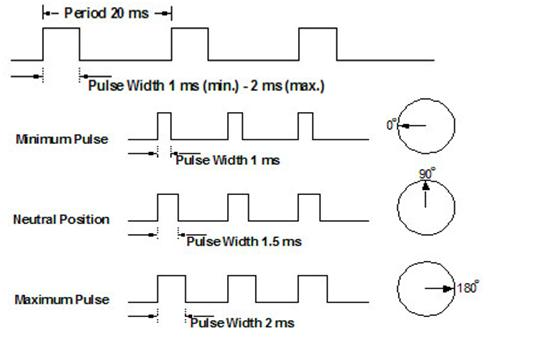
\includegraphics[width=0.8\textwidth]{img/pwm_servo.jpg}
\caption{PWM-servo kontrollsignal \cite{PWM}}
\label{fig:PWM}
\end{figure}   

\subsubsection{Gyrometer}

Et gyrometer er en innretning som kan måle vinkelposisjoner i forhold til et gitt plan. Gyrometer brukes i mange sammenhenger og finnes i mange varianter, men i denne rapporten vil kun gyrometer av typen MEMS bli beskrevet. 

Et MEMS-gyrometer (Micro Electro-Mechanical System) er lite og lett, og integreres i pakker som likner pakningene til integrerte kretser. Dette gjør at MEMS-gyrometerer enkelt kan legges på kretskort sammen med annen elektronikk. Et MEMS-gyrometer består av en stav, laget i mikromekanikk, ofte formet som en stemmegaffel. Når spenning påføres vil de to tinderene vibrere i motsatt retning av hverandre. Hvis hele staven dreies i en ny retning vil tinderne bli påført motsatt rettet kraft og kapasitansen mellom dem vil da endre seg. Denne kapasitansendringen kan måles og det er dermed mulig å detektere om legemet endrer orientering.\cite{MEMS}

MPU-6050 fra Invensense, som ble brukt i dette prosjektet, er et 6-akset gyrometer og akselerometer som gir ut data digitalt. Det har en innebygd 10-bit ADC og bruker en $I^{2}C$-buss for å kommunisere med andre enheter.\cite{InSens}

\subsection{Hardware}
For å kunne styre riggen er det nødvendig å ha en datamaskin ombord i flyet. Det finnes en rekke alternativer på dette området, men her vil Arduino og Raspberry Pi bli presentert. Hovedoppgaven til datamaskinen er å få data fra kameraet, og orientere riggen etter disse. Datamaskinen må også kunne håndtere flere prosessorer uten at det blir konflikt mellom dem. På presantasjonen til Kongberg kom det frem at de ville benytte seg av en egen GPU til bildebehandling. Men de kunne også tenke seg en samlet løsning hvor all funksjonaliteten er samlet på en chip.

\subsubsection{Arduino}
Arduino er en open source utviklingsplattform basert på \textit{ATmega328}, en 8-bits mikrokontroller fra Atmel. Bruksområdet er hovedsakelig hobbyprosjekter og prototyping. Kortet har 14 digitale porter og 6 analoge inn-porter, som vist i figur \ref{fig:Arduino}. Seks av de digitale portene kan sende PWM-signaler. Siden servomotorer bruker disse signalene er det mulig å koble opp til 6 servomotorer til en Arduino. 

\begin{figure}[h!]
\centering
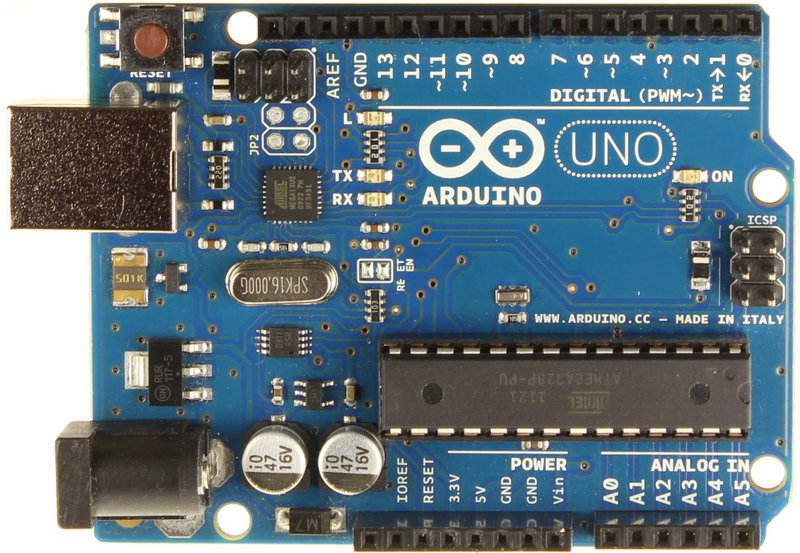
\includegraphics[scale = 0.25]{img/arduinoBoard.jpg}
\caption{Arduino Uno R3 \cite{Arduino}}
\label{fig:Arduino}
\end{figure}

Arduino programmeres i C++, og programmene overføres til kortet via USB. USB-porten på kortet kan også benyttes som COM-port, slik at Arduinoen kan ta inn eksterne kommandoer. Disse kommandoene kan for eksempel være vinkler som en servomotor skal innstilles til. På mikrokontrolleren er det også installert et lite operativsystem som inneholder en rekke biblioteker som gjør at abstraksjonsnivået blir høyere enn ordinær AVR-programmering. Det er for eksempel ikke nødvendig å endre bits i dataregistre da bibliotekene håndterer dette. 

\subsubsection{Raspberry Pi}
\label{sec:Pi}
Raspberry Pi er en minidatamaskin basert på en 32-bits ARM-arkitektur. Linux er installert på et SD-kort, og all programmering skjer direkte på Raspberry Pi. Maskinen kan brukes ved å koble den til en monitor via HDMI, eller ved å koble den til Internett via nettverksporten og koble seg til via SSH fra en annen datamaskin. Kortet har 8 I/O-pinner, som kan brukes til seriell kommunikasjon. Den er også utstyrt med 2 USB-porter, slik at en for eksempel kan koble til et kamera. En presentasjon av Raspberry PI er gitt i figur [\ref{fig:Raspberryfigur}].

\begin{figure}[h!]
\centering
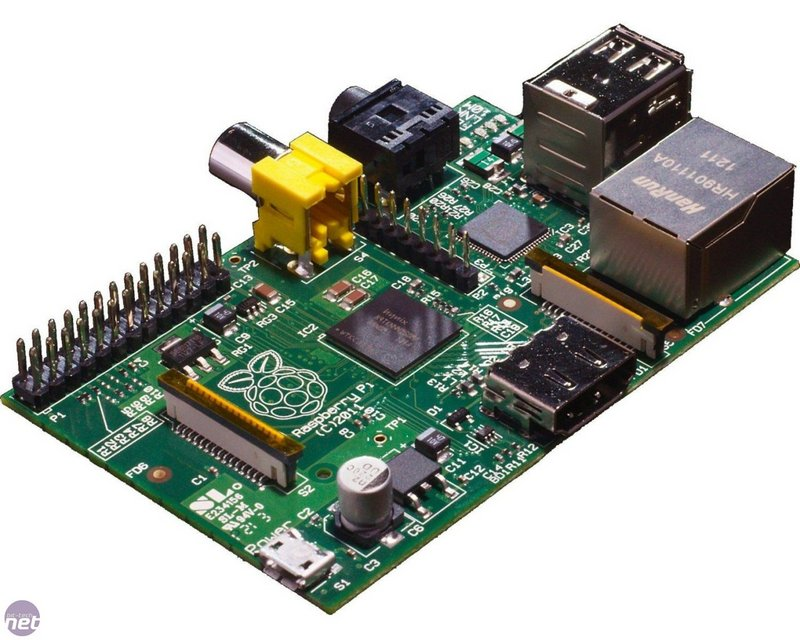
\includegraphics[scale = 0.25]{img/pi.jpg}
\caption{Raspberry Pi Model B \cite{Raspberry}}
\label{fig:Raspberryfigur}
\end{figure}  

\newpage
\subsubsection{Sammenligning mellom Arduino og Raspberry Pi}
En sammenlikning mellom Arduino Uno og Raspberry Pi model B er gitt i tabell [\ref{tab:ArdRas}]

\begin{table}[H]
\caption{Sammenligning mellom Arduino og Raspberry Pi \cite{ArduinoSpec,RpiSpec}}
\centering
\begin{tabular}{ |c |c |c| }
	\hline
   & Arduino & Raspberry Pi \\
	\hline
  	CPU & 	ATmega328 & ARM1176JZF-S \\
  	Klokkehastighet & 16 MHz & 700 MHz \\
	Minne & 32KB & 512MB\\ 
	CPU-størrelse & 8bit & 32bit\\
	I/O-porter & 14 & 8 \\
	PWN-porter & 6 & 1 \\
	USB-porter & 1 & 2 \\
	Strømforbruk & 250mW & 3.5W\\
	Pris & \$26 & \$35 \\
	\hline  
\end{tabular}
	\label{tab:ArdRas}
\end{table}

Med tanke på spesifikasjoner er Raspberry Pi mye kraftigere enn Arduino Uno med klart raskere prosessor og mye større minne. En annen fordel er at Raspberry Pi inneholder en GPU, noe Arduino Uno ikke gjør. Dette betyr at Raspberry Pi potensielt kan utføre bildegjenkjenning og styre servoene samtidig. På den andre siden har Raspberry Pi kun én PWM-port, noe som betyr at hvis denne skal styre servoer må to I/O-porter implementeres som PWM-porter i software. Dette vil resultere i mer programmeringsarbeid. En annen ulempe med Raspberry Pi i forhold til Arduino er strømforbruket som er 140\% høyere ved stand-by.\cite{ArduinoSpec,RpiSpec} Kongsberg påpeker også at de kan sende opp en egen GPU i flyet, som betyr at bildegjenkjenningen kan gjøres på denne. Med dette i tankene falt valget på Arduino Uno for å kontrollere servoene.

\subsubsection{Kommunikasjonsprotokoll}

Som nevnt kan det sendes kommandoer til Arduino kortet serielt gjennom en serieport, som også kalles en UART. Det finnes to slike serieporter på Arduino-kortet, og disse er USB-porten og I/O-port 0 (RX) og 1 (TX). I dette prosjektet vil USB-porten bli benyttet for å kommunisere mellom en datamaskin og Arduinokortet. Fordelen med å bruke USB-porten er at det er enkelt, at alle nye datamaskiner har en USB-port og det er ikke nødvendig å lage en egen protokoll med \emph{header}, \emph{error correction} og så videre. En ulempe er at denne protokollen er standard slik at den ikke kan endres for å passe kun dette prosjektet og på denne måten minke mengde \emph{overhead}.

\subsection{Software}

Matlab brukes til å utforme matematiske modeller, utføre komplekse beregninger og visualisere data. \cite{matlab} Programmet er mye brukt i vitenskapelige miljøer og er meget anerkjent. 
OpenCV er et softwarebibliotek med åpen kildekode som brukes til digital bildebehandling. Biblioteket i versjon 2.x, som er versjonen benyttet i dette prosjektet, og er programmert i C++. \cite{docs:opencv}

For å kunne bruke funksjoner fra OpenCV i Matlab måtte mexopencv tas i bruk. Matlab er ikke uten videre kompatibelt med OpenCV, da dette er programmert i C++. Mexopencv tilbyr Matlabfunksjoner som bygger på flere hundre APIer fra OpenCV. \cite{mexopencv} Dette tillater å programmere alt i Matlab, uten å måtte fokusere på hvordan OpenCV er bygget opp. 
